\section{Methodology}

To better understand ET's role in future contextual AI systems, we first estimate the ET signal quality needed for accurate gaze-based selection of physical objects.  Next, to measure the ability of AI agents to incorporate ET context, we experiment with end-to-end contextual AI tasks.  We inject contextual cues derived from the user's eye gaze into VLM queries, improving the model's ability to understand user attention and current actions.

\subsection{Eye tracking requirements for registering nearby objects}

Contextual AI models that collaborate with users would benefit from knowledge of users' real-world interests.  ET is a promising signal to capture the user's attention, both at one point in time~\cite{konrad_gazegpt_2024}, or continuously to build historical context.  We hypothesize that the visual angle subtended by objects that users ``look at'' defines a lower bound on ET signal accuracy.  By measuring the visual angle expressed by nearby objects, we can approximate the ET accuracy required to consistently track a user's point of focus.

To investigate accuracy requirements, we analyze objects that are nearby in the user's field of view (FOV) during daily household tasks, then relate the object size statistics to ET signal quality requirements.  Because we expect humans and AI agents to collaborate in daily life, it is important for the ET system to achieve an accuracy which allows consistent, accurate attention modeling in a broad set of scenarios~\cite{feit2017toward}.  Individuals are far more likely to look at or interact with objects in the immediate vicinity~\cite{ballendat_proxemic_2010}, so we constrain this analysis to objects which are nearby candidates for interaction.

\subsubsection{Dataset}

For our analyses, we use a subset of the Aria Digital Twins (ADT) dataset~\cite{pan_adt_2023}.  The ADT dataset contains egocentric recordings of daily-life tasks in indoor environments.  We analyze single-participant recordings in the fully furnished apartment scene (93 recordings), totaling $\sim$3 hours of footage.  Designed to model real-world household scenarios, these recordings span the following tasks:  decorating, cooking, working, cleaning, and object examination.

In addition to the ET signal (median error $= 1.5\degree$) provided by Project Aria glasses~\cite{engel_aria_2023}, the ADT dataset contains ground-truth information about physical objects in the scene.  Each object's position, orientation, bounding box, and segmentation region is tracked and available throughout a recording, with median tracking error of $5 mm$.  This ground-truth data uniquely enables us to analyze object visual statistics at a fine scale, detect human-object interactions, and accurately place gaze on objects.  396 household objects are tracked in the dataset, with varying presence across different tasks and recordings.

\subsubsection{Object visual size in relation to eye tracking error}

\begin{figure}[t]
 \centering
 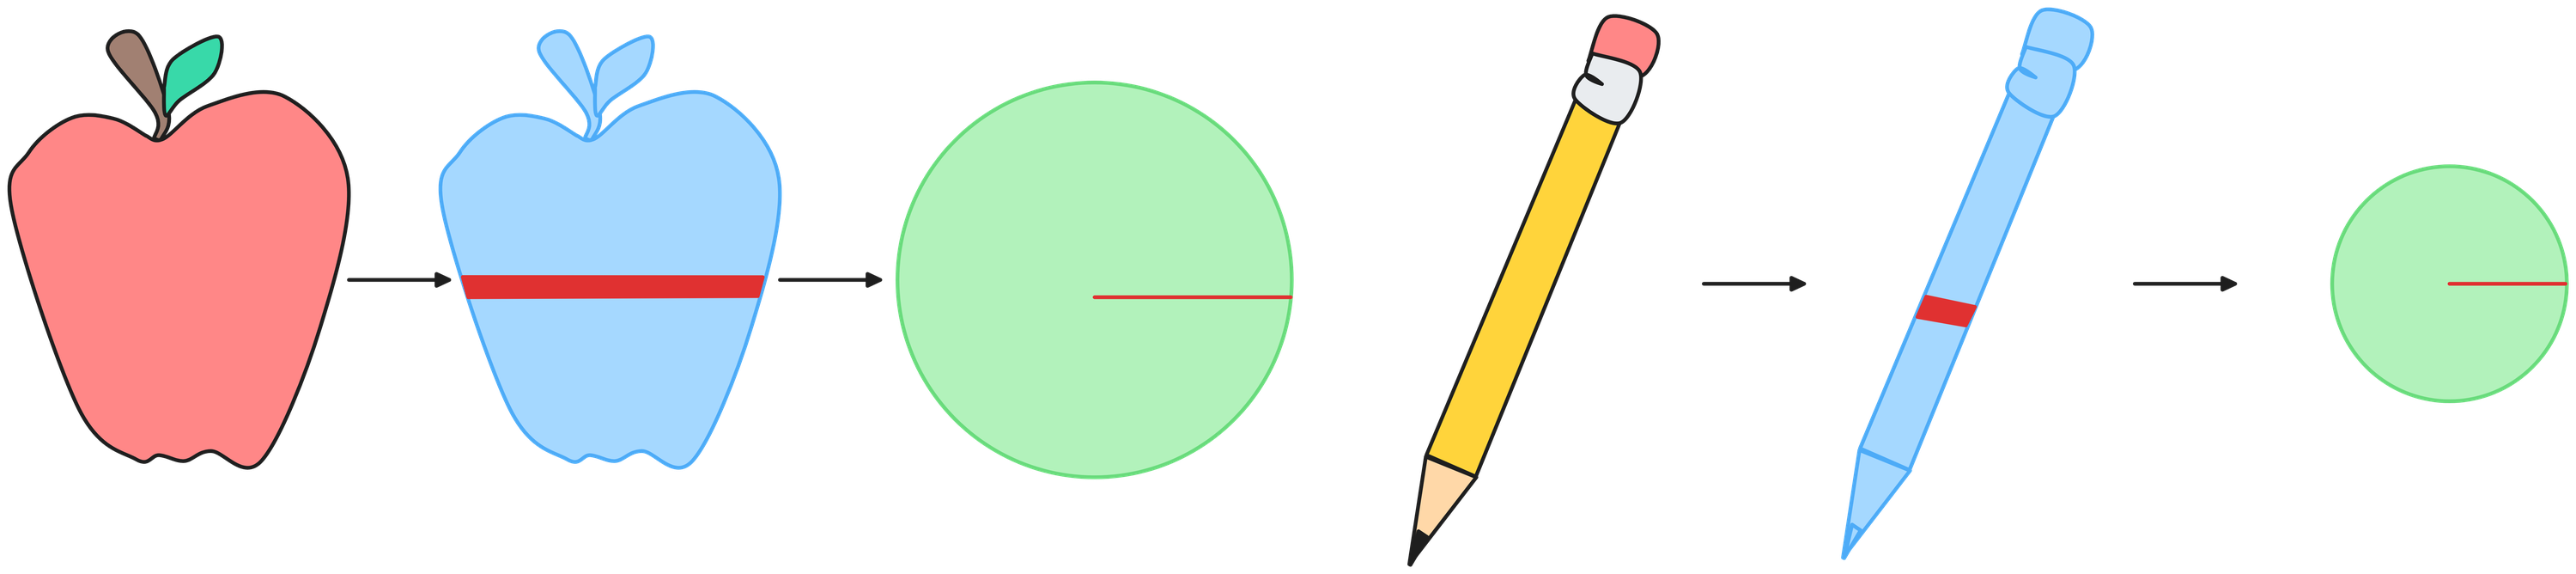
\includegraphics[width=0.5\linewidth]{figures/segment_illustration_flat.png}
 \caption{Illustration of eye tracking spatial error and object visual size measurements.  As an average case measurement, object segmentation area can be mapped to a circular region, with the radius reflecting the eye tracking accuracy requirement (\textcolor{red}{thin bars}).  Alternatively, $1 / 2$ minor axis span $L_{min}$ (\textcolor{red}{thick bars}) is a tighter bound for measuring non-uniform objects.}
 \label{fig:et_relationship}
\end{figure}

ET spatial error is the measured bias between the ground truth and estimated gaze positions.  This error persists following techniques such as ET calibration and fixation detection.  We measure spatial error as an angular offset between the user's true gaze point and computed value.  We wish to approximate the influence of ET spatial error in placing fixations on object, to better inform how reliably an ET system could convey a user's attention on world objects.

Our metrics to predict ET accuracy needs are derived from object visual size, the visual angle spanned by the object relative to the user's FOV.  Visual size is related to both the physical size of an object and its distance from the user.  We approximate object visual size from the total segmentation area $A_{{}_{seg}}$ of an object in a linear camera model (measuring degrees$^2$ occupied by the object).  To convey visual size against an ET error requirement $err_{{}_{ET}}$, we convert visual size to the approximate \textbf{radius} of the object. $err_{{}_{ET}} \ \leq \ \sqrt{A_{{}_{seg}} / \pi}$.  This inequality approximates an \textbf{average case} need for ET error requirement, and is valid when objects have roughly uniform dimensions.  To account for non-uniform objects, we compute a more \textbf{conservative} ET error as $1 / 2$ the \textbf{minor axis} span $L_{min}$ of the object's segmentation region: $err_{{}_{ET}\ low} \ \leq \ 1 / 2 \ L_{min}$.  \autoref{fig:et_relationship} illustrates these metrics and the relationship between ET error requirements and object visual size.

\subsubsection{Protocol}

We approximate the ET requirements for daily use by observing the household tasks being performed in the ADT dataset~\cite{pan_adt_2023}.  We measure the distributions of object visual sizes for $err_{{}_{ET}}$ and $err_{{}_{ET}\ low}$.  To better inform various contextual AI applications, we specify the ET requirements across different interaction spaces, namely:
\begin{enumerate}  [topsep=0pt]
    \item \textbf{Near-field objects:} all objects within 1 meter of the participants.
    \item \textbf{Mid-field objects:} all objects between 1 - 2 meters of the participants.
    \item \textbf{Interacted objects:} all objects being physically interacted with (held, pressed, pushed, etc.) by the participants, with a start / stop padding of 1 second for the interaction.
    \item \textbf{Fixated objects:} all objects within 2 meters fixated on by participants' gaze as they navigate the scenes.
\end{enumerate}

\begin{figure}[h]
    \centering
    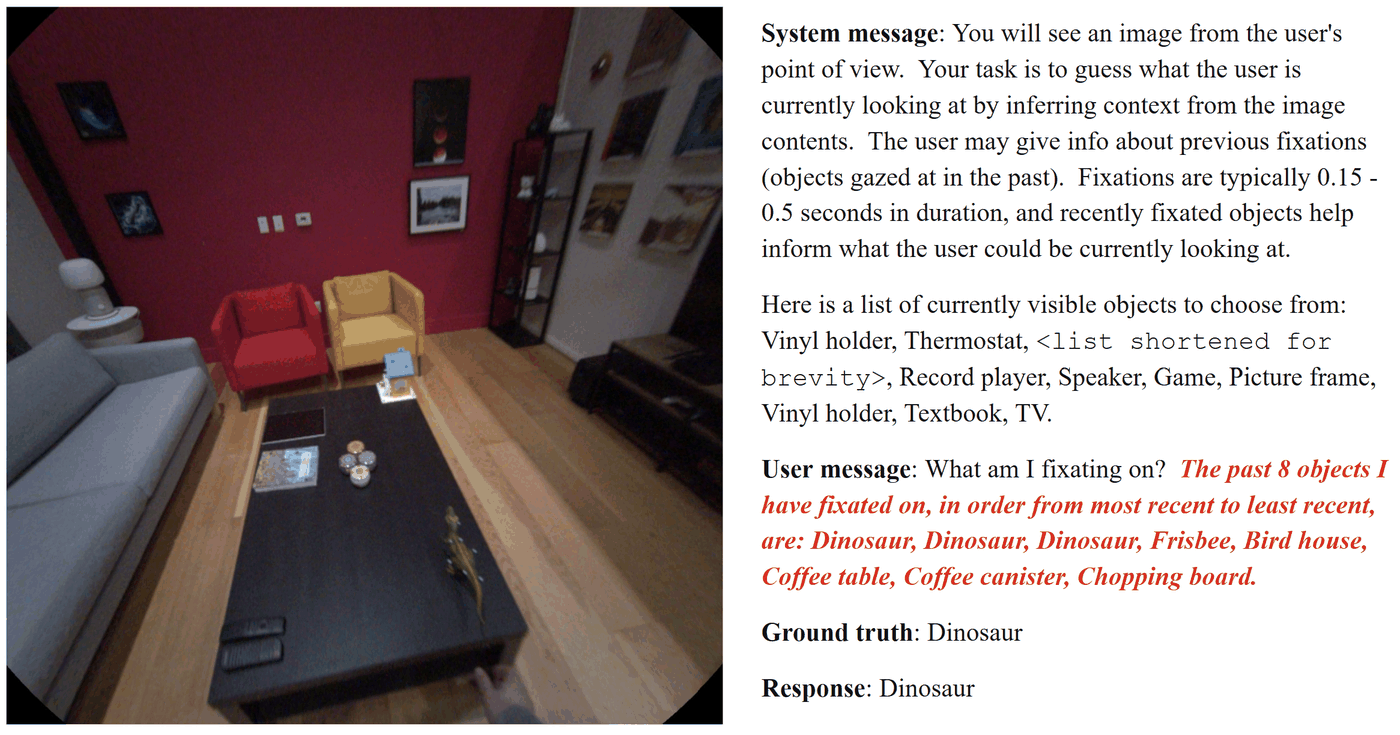
\includegraphics[width=0.9\linewidth]{figures/query_example.png}
    \caption{An example query to the VLM for E1.  The additional context from fixation history is highlighted in red; We vary the amount of context given to the model to measure how this context influences model understanding.}
    \label{fig:query_example}
\end{figure}

\subsection{Contextualizing vision-language model queries with eye tracking information}

To begin to explore the value that ET signals can provide in contextual AI systems, we model experiments which reflect potential end-to-end contextual AI systems.  In these experiments, we build up historical context by creating timelines of past fixations on physical objects.  We include this context in VLM queries and measure the positive impacts on model understanding.  Our baseline comparison is a VLM query which uses only the egocentric image as added context (similar to a Ray-Ban Meta or Google Ask Photos query).

We use the Meta Llama 3.2 90B VLM\footnote{\url{https://ai.meta.com/blog/llama-3-2-connect-2024-vision-edge-mobile-devices/}}~\cite{grattafiori_llama_2024} as our contextual AI agent.  We add context to queries with an egocentric image and additional prompting.  In both experiments, the agent is constrained via JSON to respond with one option from all currently visible objects, as we are operating under the pretense that in a full system, an object recognition / scene understanding model would be available.  Note that this VLM is not fine-tuned, and that a model tuned for egocentric image understanding and / or for a specific task would likely see improved results.  Yet, these experiments indicate the added value when incorporating ET contextual information.

\subsubsection{E1: ``What am I looking at?" with historical context.}

In this experiment, we pose the question ``what am I looking at?"  This experiment serves as a benchmark for the effect that prior eye gaze context serves in improving image understanding.  We first detect and localize fixations on objects\footnote{We use a velocity-thresholding algorithm at 100$\degree$ per second~\cite{salvucci_fixations_2000}, to account for the relatively low sampling rate of Project Aria glasses (30Hz)~\cite{engel_aria_2023}.  We only consider fixations $\geq$ 150 ms for analysis.}, then perform uniform random sampling across each recording in the ADT dataset to analyze 919 image frames which each contain at least 10 prior fixations.  At each sample, we make multiple queries, varying the number of prior fixations supplied as context to the VLM, between 0 - 10.  An example prompt set can be seen in~\autoref{fig:query_example}.

\subsubsection{E2: "What am I going to interact with?" with historical context.}

We query the VLM ``what am I going to interact with?" while again varying the amount of gaze context.  In this experiment, we supply the image from a current fixation, where a physical interaction is guaranteed to occur within the next second and at least 10 prior fixations exist (237 distinct image frames).  The vast majority of physical interactions in ADT are grasping, pushing, and pulling with hands.  This task models the use of ET as supporting context for user action understanding and prediction.

% \subsubsection{E3: Gaze-based context cropping.}

% In this experiment, we pose a similar question to E1 (``What am I looking at?"), but instead of providing historical context, we use the eye tracking signal to narrow down the visible region of the image supplied to the model.  This experiment models ET's efficacy in narrowing contextual image cues, preventing misunderstandings from objects which are not near the user's current point of gaze.  We then perform an ablation where we artificially degrade the eye tracker's accuracy, adding noise in a random direction before cropping and querying the VLM.